%%
%%                  TEMPLATE for Math 436 project report
%%
\documentclass[11pt]{amsart}
%%% WARNING: Do NOT change the page size, fonts, or margins!  Penalties will apply.


\usepackage{graphicx}
\usepackage{amssymb,amsmath,amsthm}
\usepackage{placeins} %enables \FloatBarrier, which prevents figures and tables from going below it.
\usepackage{hyperref} %makes cross references into hyperlinks. 

 

%%% WARNING: Do NOT change the page size, fonts, or margins!  Penalties will apply.
%%% WARNING: Do NOT change the page size, fonts, or margins!  Penalties will apply.

\begin{document}

\title{Flowering Plant--Caterpillar--Pollinator Predator-Prey System}
\author{Isabella Squire, Ashtyn Whipple, Tristen Turlington}

% Change the date to match the date you actually wrote this paper
\date{4 November 2026} % or use \today

\maketitle % this actually makes the title

\begin{abstract}
In this paper, we explore ODE-based models for the fluctuations of plant, caterpillar, and bee populations. We begin with a classic plant--caterpillar model (which follows the structure of a predator--prey system) and then extend it by adding a third species. Bees enter the model as mutualists. By incorporating carrying capacity, density-dependent competition among bees, and species interaction rates, we analyze the model's equilibria, their stability, and the resulting population dynamics. We then use our model to explore possible human interventions and compare their effectiveness in supporting plant growth.
\end{abstract}

%% First Section
\section{Background/Motivation}

Plants support ecosystems by providing food for consumers and releasing oxygen through photosynthesis~\cite{johnson2016}. Therefore, conserving struggling plant populations is essential and requires interventions that support plants without eliminating other species. Caterpillars consume plant leaves through herbivory~\cite{grant2022}, which can reduce plant growth and place additional pressure on vulnerable populations. Bees, in contrast, have a mutualistic relationship with flowering plants: they collect nectar and pollen while transferring pollen between flowers, helping plants reproduce~\cite{revilla2015}. These opposing effects raise the question of whether supporting bees can compensate for plant loss from caterpillars.

We model these interactions to investigate how plants, caterpillars, and bees respond to possible interventions. We begin with a plant--caterpillar model based on the established Lotka--Volterra predator--prey framework, modified to include logistic plant growth~\cite{grunert2021}. We then introduce bees through mutualistic terms representing the benefits of pollination to plants and floral resources to bees.

Conservation and management efforts include reducing excessive herbivory and supporting pollinator populations~\cite{fwsIntegratedPestManagement,epaPollinatorProtection}. We simulate these approaches to compare their effectiveness in maintaining plant abundance. Through these comparisons, we aim to help conservation practitioners understand which strategies could provide lasting support under the conditions represented by our model. Our goal is to identify approaches that benefit plants while allowing all three populations to coexist.

\subsection{Related Work}

Previous research has combined plant growth, herbivory, and pollination by modeling an insect that feeds on plants as a larva and pollinates as an adult~\cite{revilla2015}. Our model instead treats bees and caterpillars as separate populations and compares interventions to support plant abundance.

% \begin{figure}[htb]
% \begin{center} %Put your images in a figure like this
% \includegraphics[width=\textwidth]{Myfig.pdf} % Better to make them pdfs than png or gif or jpeg
% \end{center}
% \caption{Plots should be high resolution (pdf 300dpi), uncluttered, a reasonable size, and easily readable and understandable. If you make plots in MatPlotLib, be sure to set the \texttt{figsize} option to be the actual size in inches that your final figure will be in the LaTeX document (so width 5 for a full-width figure).  Otherwise when you put your figure in your document it will scale the text to be a bad size---either too big or too small.  All figures should have a complete caption that helps the reader make sense of the figure even if they haven't read the paper yet. Here is an example: This figure shows the risk or mean squared error (in black) of for a generic family of regression models as a function of model complexity (the number of free parameters in the model).  The generalized aliasing decomposition shows that the risk is the sum of three parts: Model insufficiency (red), Data insufficiency (green), and Aliasing (blue).  Model insufficiency is monotonically decreasing as a function of complexity, Data insufficiency vanishes when the number of parameters is less than the number of training points (the classical regime), but increases monotonically in the modern regime (where the number of parameters is greater than the number of data points).  Aliasing generally increases up to the interpolation threshold and decreases thereafter, converging to zero almost surely as the number of parameters goes to infinity.  
% }
% \label{fig:MeanSquaredError} % for automatic cross referencing
% \end{figure}



%% Second Section 
\section{Modeling}

\subsection{Model 1 -- Plants and Caterpillars}

We start with Model 1, which investigates the interactions between flowering plants and caterpillars. Let (P) represent the plant population and (C) represent the caterpillar population at a given time. Plants grow naturally but are limited by the environment's carrying capacity, while caterpillars depend on plants as their food source. As the caterpillar population increases, more plants are consumed, which reduces plant growth. Caterpillars also reproduce based on the amount of available food.

We define the system of ODEs as follows:

\[
\begin{aligned}
\frac{dP}{dt} &= r P\left(1-\frac{P}{K}\right)-aPC \\[6pt]
\frac{dC}{dt} &= -\mu C+\varepsilon aPC
\end{aligned}
\]

Here, $r$ represents the plant growth rate, $K$ is the plant carrying capacity, and $a$ represents the rate at which caterpillars consume plants. The parameter $\mu$ represents the caterpillar death rate, while $\varepsilon$ represents the efficiency with which consumed plants contribute to caterpillar reproduction. This model allows us to evaluate how plant carrying capacity and the interactions between caterpillars and flowering plants affect the survival of both populations.

The model has three possible equilibria, representing extinction of both populations, plants surviving without caterpillars, and coexistence of both species. These equilibria are:

\[
E_0=(0,0), \qquad E_P=(K,0),
\]

\[
E_{PC}=
\left(
\frac{\mu}{\varepsilon a},
\frac{r}{a}\left(1-\frac{\mu}{\varepsilon aK}\right)
\right).
\]

The coexistence equilibrium is biologically feasible when

\[
K>\frac{\mu}{\varepsilon a}.
\]

This condition indicates that the plant carrying capacity must be sufficiently large to support both populations. The extinction equilibrium is a saddle point, while the plant-only equilibrium is stable below this threshold. Above the threshold, the coexistence equilibrium is stable. These results show that the model can represent several realistic ecological outcomes, including extinction, plant survival without herbivores, and coexistence between plants and caterpillars.

Model 1 describes the interactions between flowering plants and caterpillars but does not account for the role of bees in pollination. Since bees contribute to plant reproduction and growth, their presence may also indirectly affect caterpillar populations by changing food availability. Therefore, we extend the model by adding bees to investigate how pollination influences plant growth and the balance between all three populations.

\subsection{Model 2 -- Plants, Caterpillars, and Bees}

Let $B$ represent the bee population. Bees visit flowering plants to collect nectar and pollen, which supports their population growth while also helping plants reproduce. We define the system as follows:

\[
\begin{aligned}
\frac{dP}{dt} &= rP\left(1-\frac{P}{K}\right)-aPC
+\beta\frac{vPB}{H+P}\left(1-\frac{P}{K}\right) \\[6pt]
\frac{dC}{dt} &= \varepsilon aPC-\mu C \\[6pt]
\frac{dB}{dt} &= \gamma\frac{vPB}{H+P}-dB-qB^2
\end{aligned}
\]

We model the additional growth that bees bring to flowering plants as $\beta\frac{vPB}{H+P}\left(1-\frac{P}{K}\right)$. The flower visitation component, $\frac{vPB}{H+P}$, is a saturating, Michaelis--Menten-like term~\cite{mcpeek2022}, where $v$ is the maximum flower visitation rate per bee and $H$ is the plant abundance at which visitation reaches half its maximum. This allows visitation to increase with plant abundance while eventually saturating, since a bee cannot visit an unlimited number of flowers. Each bee visit contributes to plant reproduction through the parameter $\beta$, with the additional factor $1-\frac{P}{K}$ keeping plant growth limited by carrying capacity.

We retain logistic plant growth without bees, assuming that some baseline growth and reproduction can occur independently of the bee population represented in our model. The caterpillar equation remains the same as in Model 1.

We then add an equation for the bee population. We again represent flower visitation by $\frac{vPB}{H+P}$ and multiply it by $\gamma$, the contribution of flower visits to bee population growth. Finally, $d$ represents the natural bee mortality rate, and $q$ controls the strength of competition among bees. The $B^2$ term makes losses from competition increase more rapidly as the bee population grows.


This model has 5 nonnegative equilibria, listed in the order $(P,C,B)$. For simplicity, we write $P^*=\mu/(\varepsilon a)$ and $B^*=\bigl(\gamma vP^*/(H+P^*)-d\bigr)/q$:
\begin{align*}
E_0 &= (0,0,0), \\
E_P &= (K,0,0), \\
E_{PC} &= \left(P^*,\frac{r}{a}\left(1-\frac{P^*}{K}\right),0\right), \\
E_{PB} &= \left(K,0,\frac{1}{q}\left(\frac{\gamma vK}{H+K}-d\right)\right), \\
E_{PCB} &= \left(P^*,\frac{1}{a}\left(1-\frac{P^*}{K}\right)
\left(r+\frac{\beta vB^*}{H+P^*}\right),B^*\right).
\end{align*}
The extinction, plants-only, and plant--caterpillar equilibria correspond to those of Model 1 with no bees. The plant--bee equilibrium $E_{PB}$ and three-population coexistence equilibrium $E_{PCB}$ are new outcomes introduced by adding bees.

The three-population coexistence equilibrium requires
\[
K>\frac{\mu}{\varepsilon a}
\qquad\text{and}\qquad
\frac{\gamma vP^*}{H+P^*}>d.
\]
The first condition is the same carrying-capacity requirement as in Model 1; the additional condition requires sufficient plant resources for bee reproduction to exceed natural mortality. Unlike Model 1, however, biologically feasible coexistence is not automatically stable for every parameter choice in Model 2. For our chosen parameters, coexistence is stable throughout the sampled range $125<K\leq200$, matching Model 1's stable coexistence behavior over this range.






%% Third Section
\section{Results}

\subsection{Parameter Values}
Parameter values were estimated from published literature studies and held fixed across all simulations unless specified. The parameters $r$, $K$, $a$, $\mu$, $v$, $\beta$, and $d$ were derived directly from sources. We did not find direct estimates for $\varepsilon$, $H$, $\gamma$, and $q$, so we estimated these parameters using the available literature and chose values that allow a stable, positive equilibrium.

\subsection{Model 1}
\leavevmode\par

\begin{figure}[!htb]
\centering
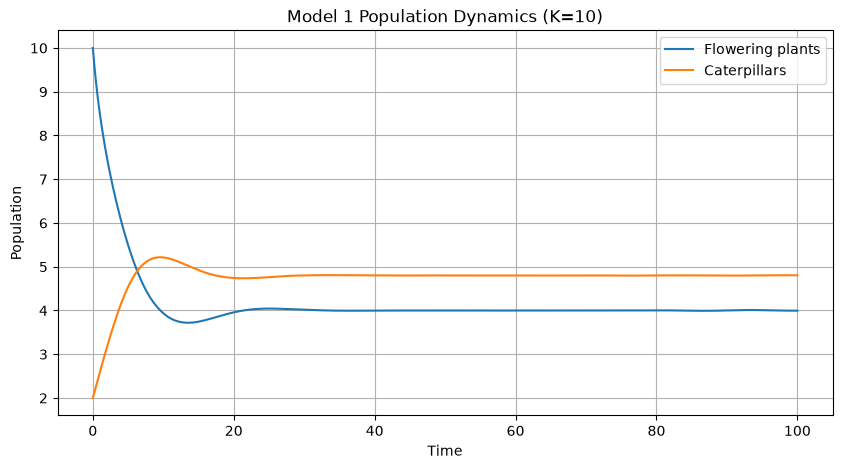
\includegraphics[width=0.8\textwidth]{model 1 population dynamics.png}
\caption{Plot for Model 1 showing how the populations of the caterpillars and the plants change with each other.}
\label{fig:model1-dynamics}
\end{figure}

\begin{figure}[!htb]
\centering
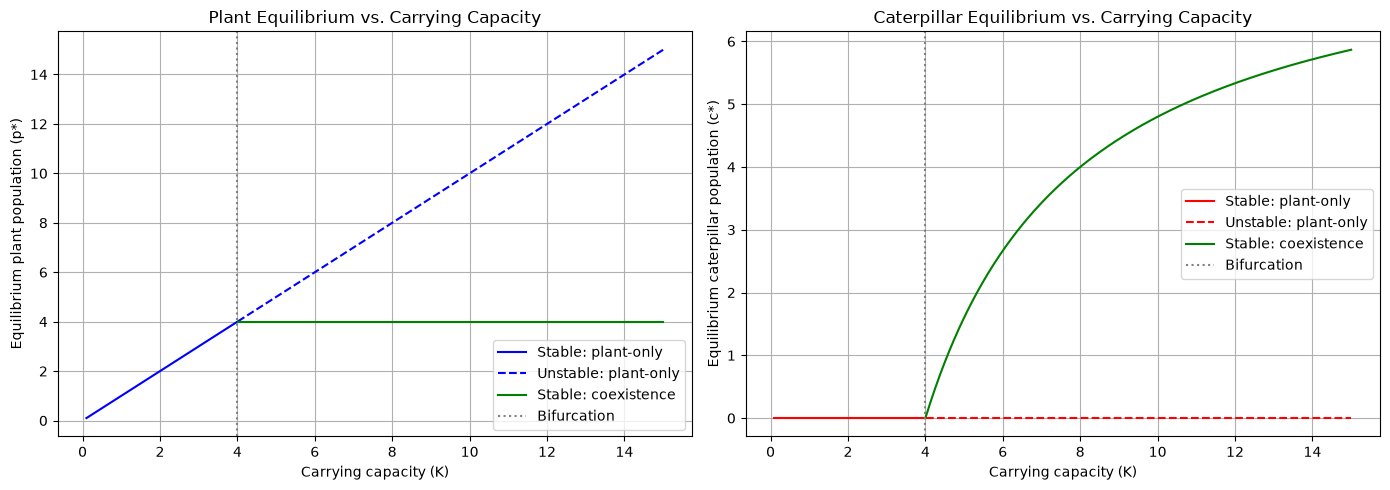
\includegraphics[width=0.8\textwidth]{model 1 bifurcation.png}
\caption{Bifurcation diagram for Model 1 showing the change in equilibrium populations as carrying capacity increases. Solid lines indicate stable equilibria, and dashed lines indicate unstable equilibria.}
\label{fig:model1}
\end{figure}

The bifurcation diagrams show how the equilibrium populations change in both stability and existence as the plant carrying capacity ($K$) increases. When $K$ is below the threshold $\frac{\mu}{\varepsilon a}=125$, the plant-only equilibrium is stable, meaning caterpillars cannot maintain a population. As seen in Figure~\ref{fig:model1}, once $K$ exceeds this threshold, a stable coexistence equilibrium becomes possible, allowing both plants and caterpillars to survive. The time-course plot (Figure~\ref{fig:model1-dynamics}) illustrates this behavior by showing both populations approaching their coexistence equilibrium values over time with $K$ = 200.

Note that for $K=200$, Figure 2 shows that the coexistence equilibrium is stable, with a plant population of 125 and a caterpillar population of approximately 4. 

\FloatBarrier

\subsection{Model 2}
\leavevmode\par

\begin{figure}[!htb]
\centering
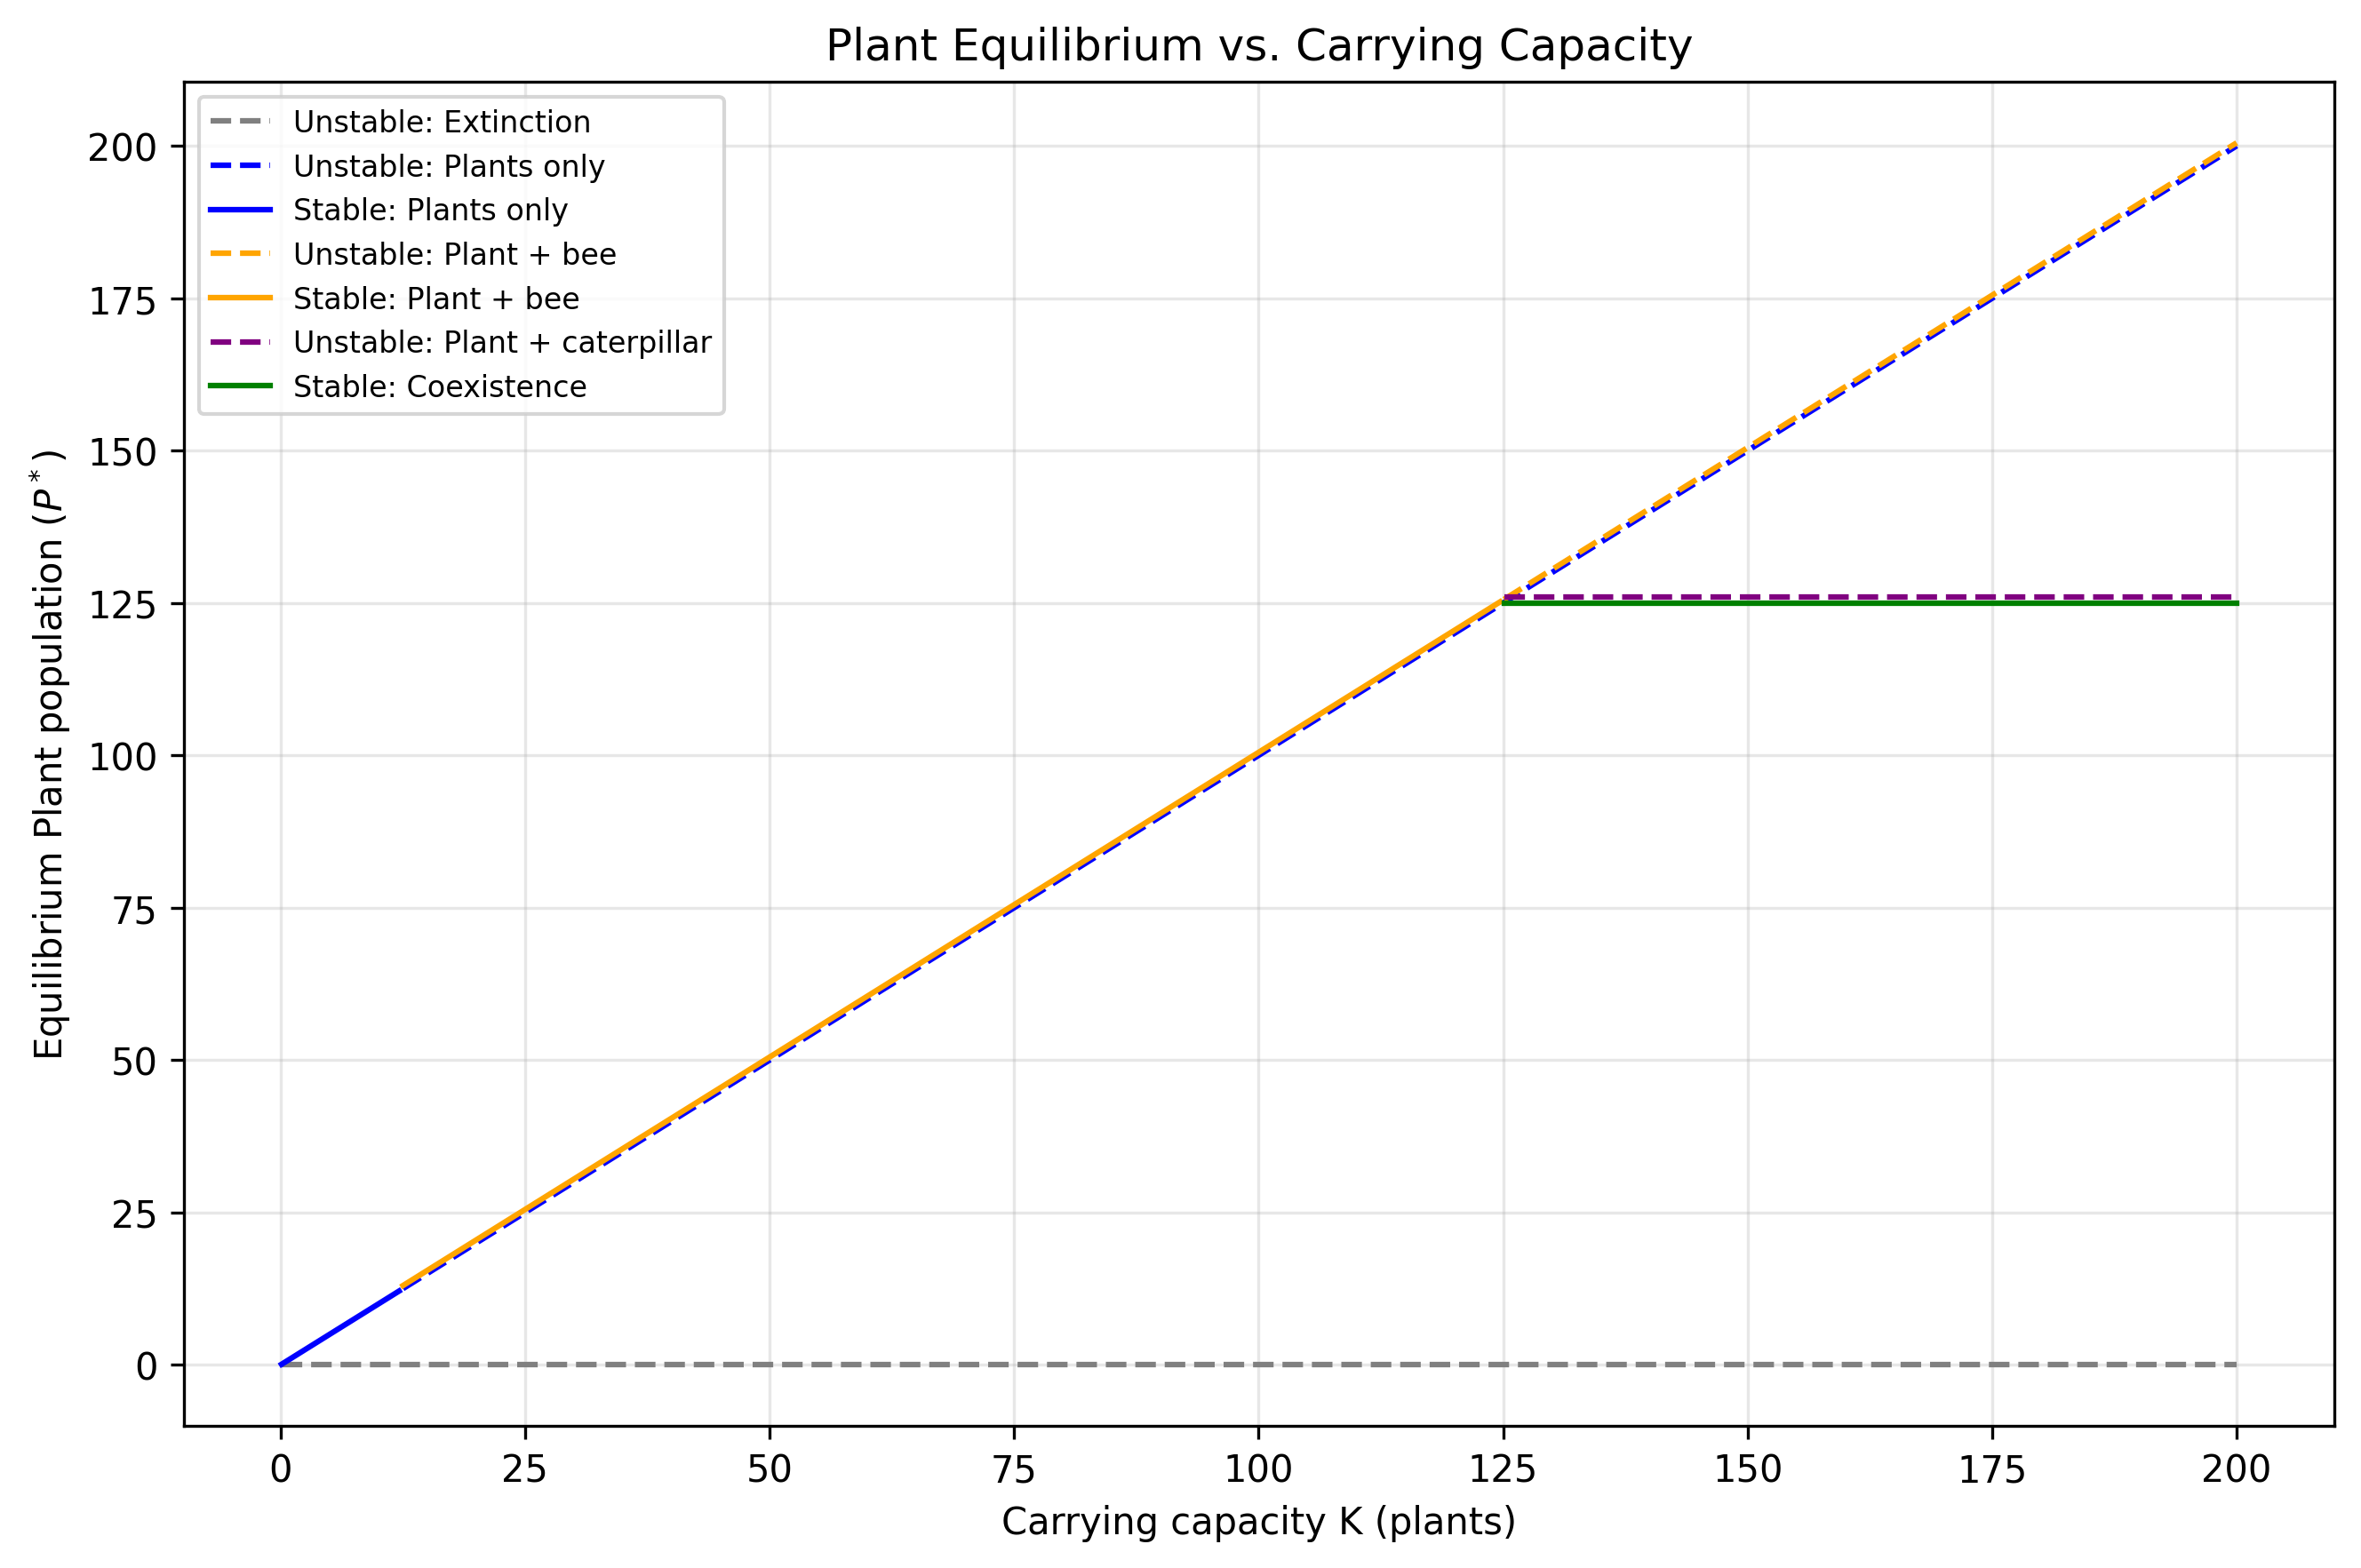
\includegraphics[width=0.48\textwidth]{model2_plants.png}
\hfill
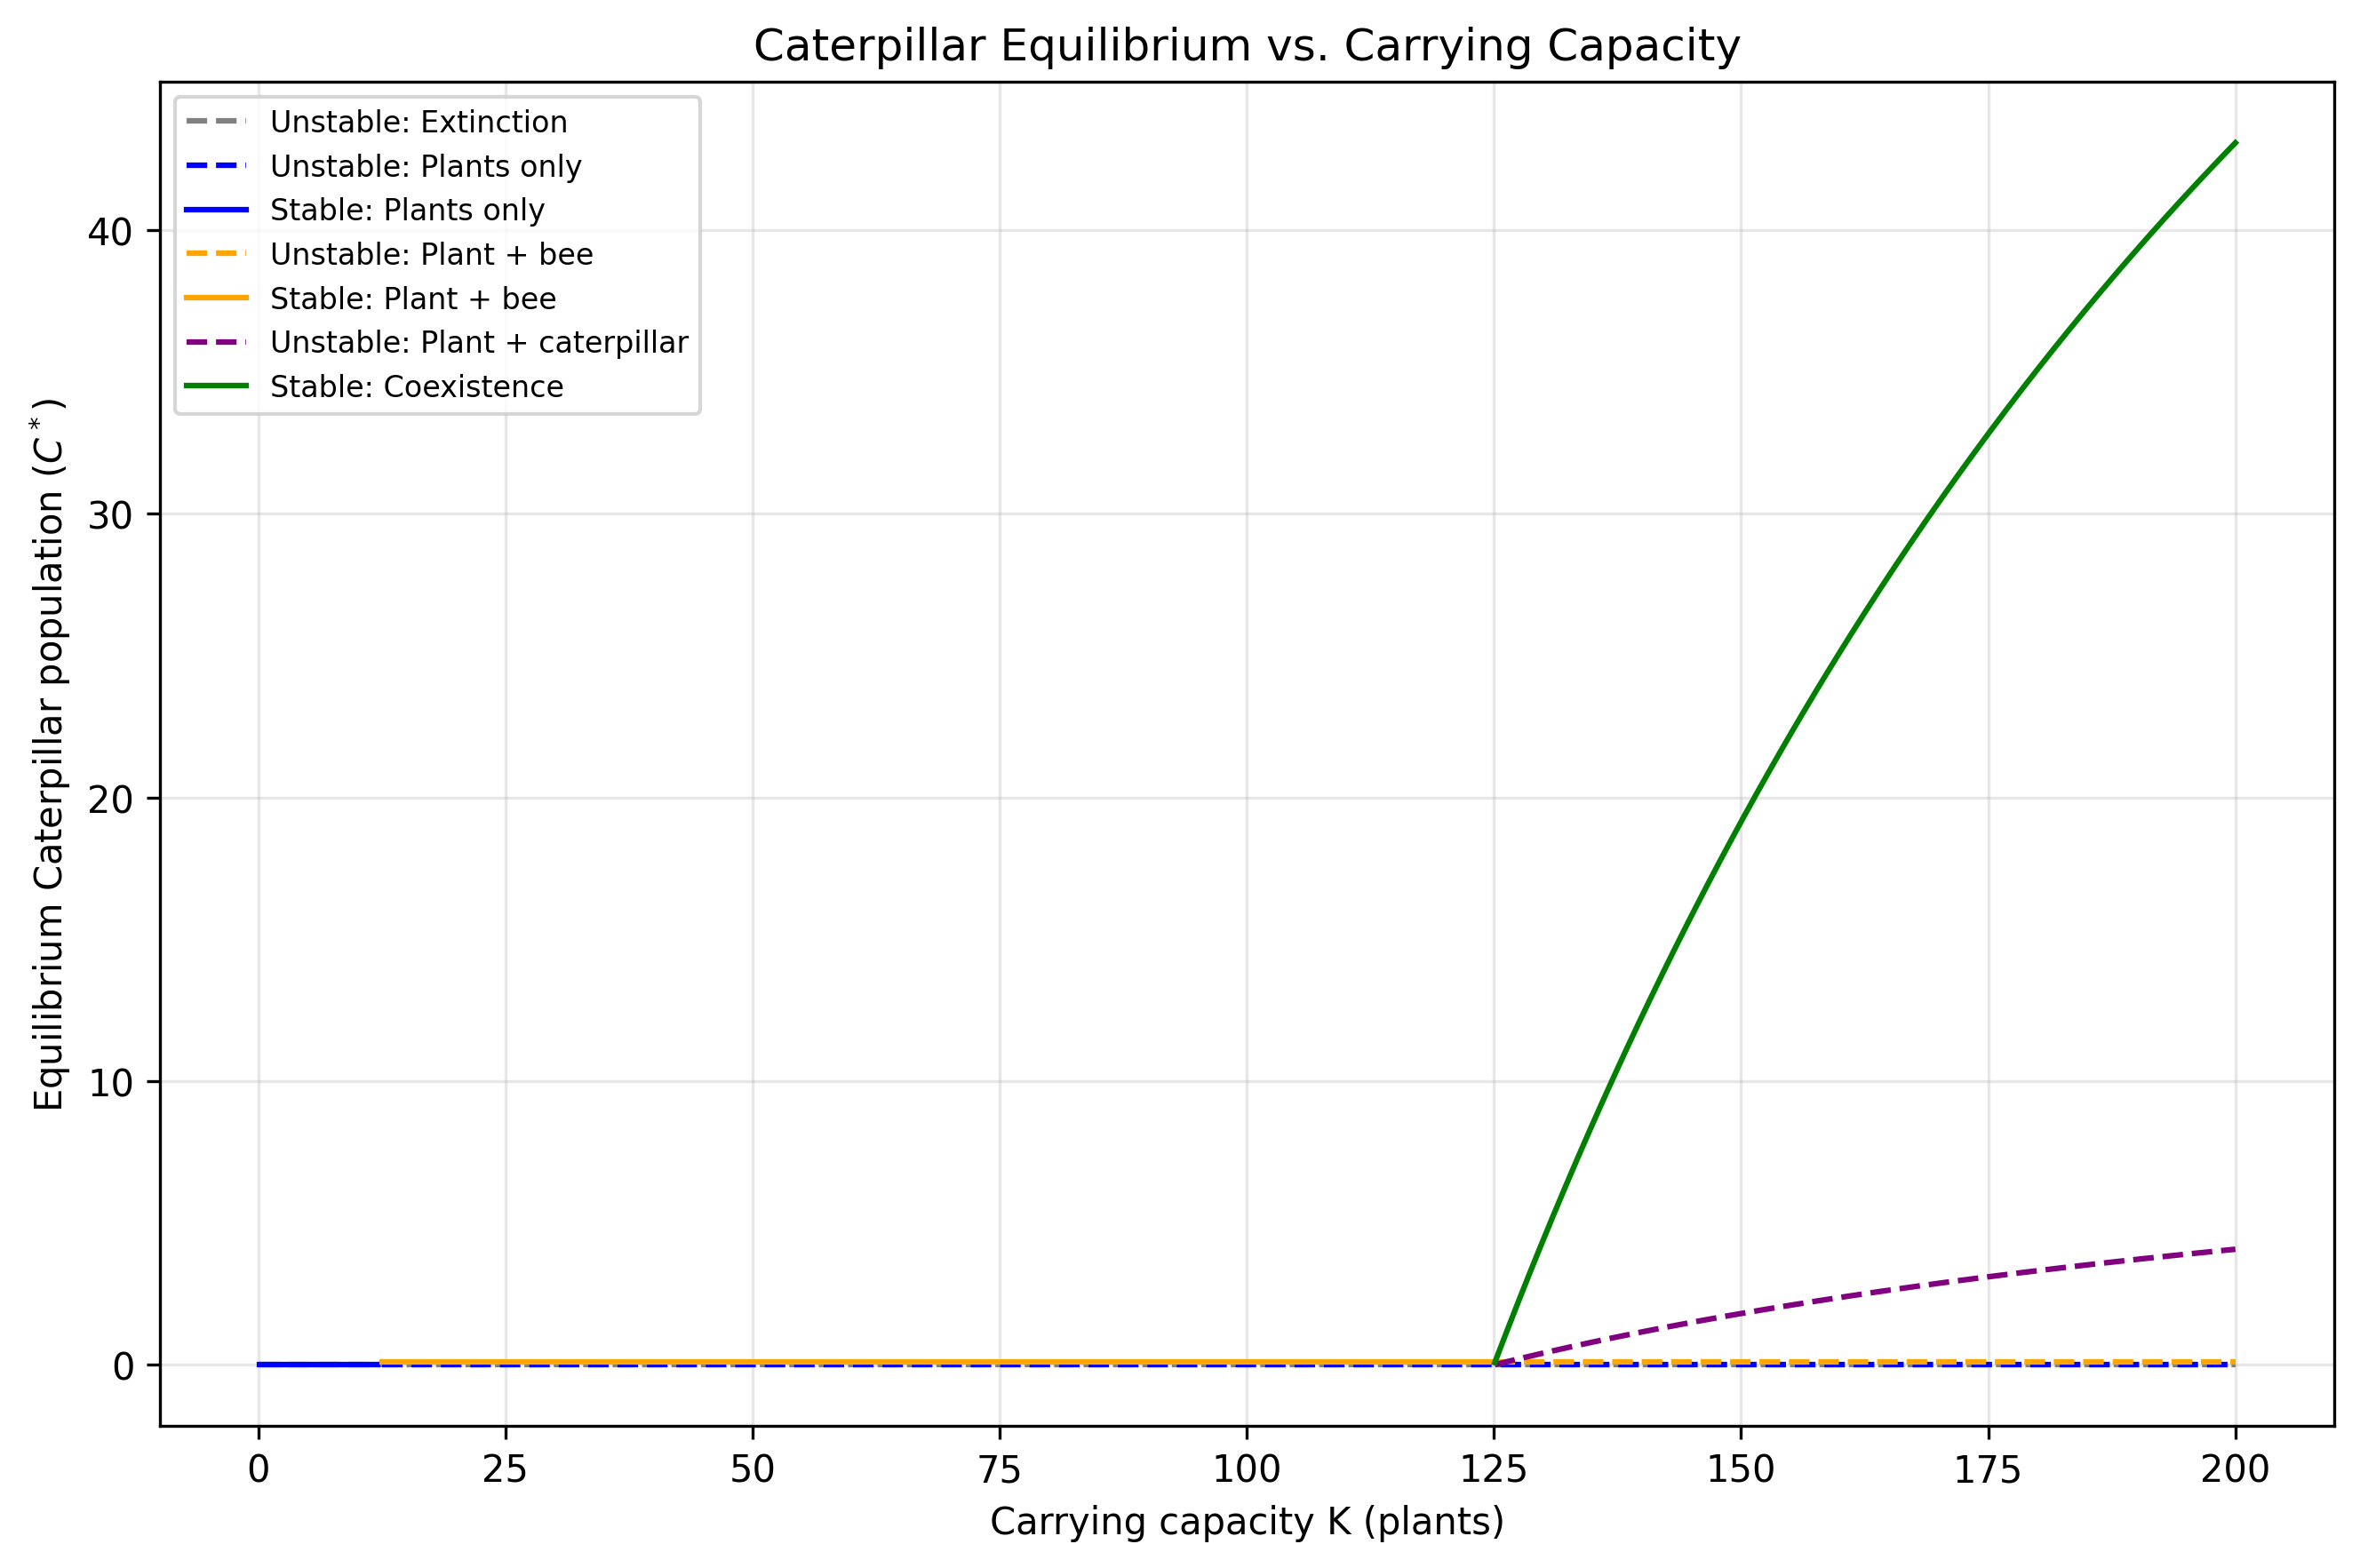
\includegraphics[width=0.48\textwidth]{model2_caterpillars.png}

\medskip
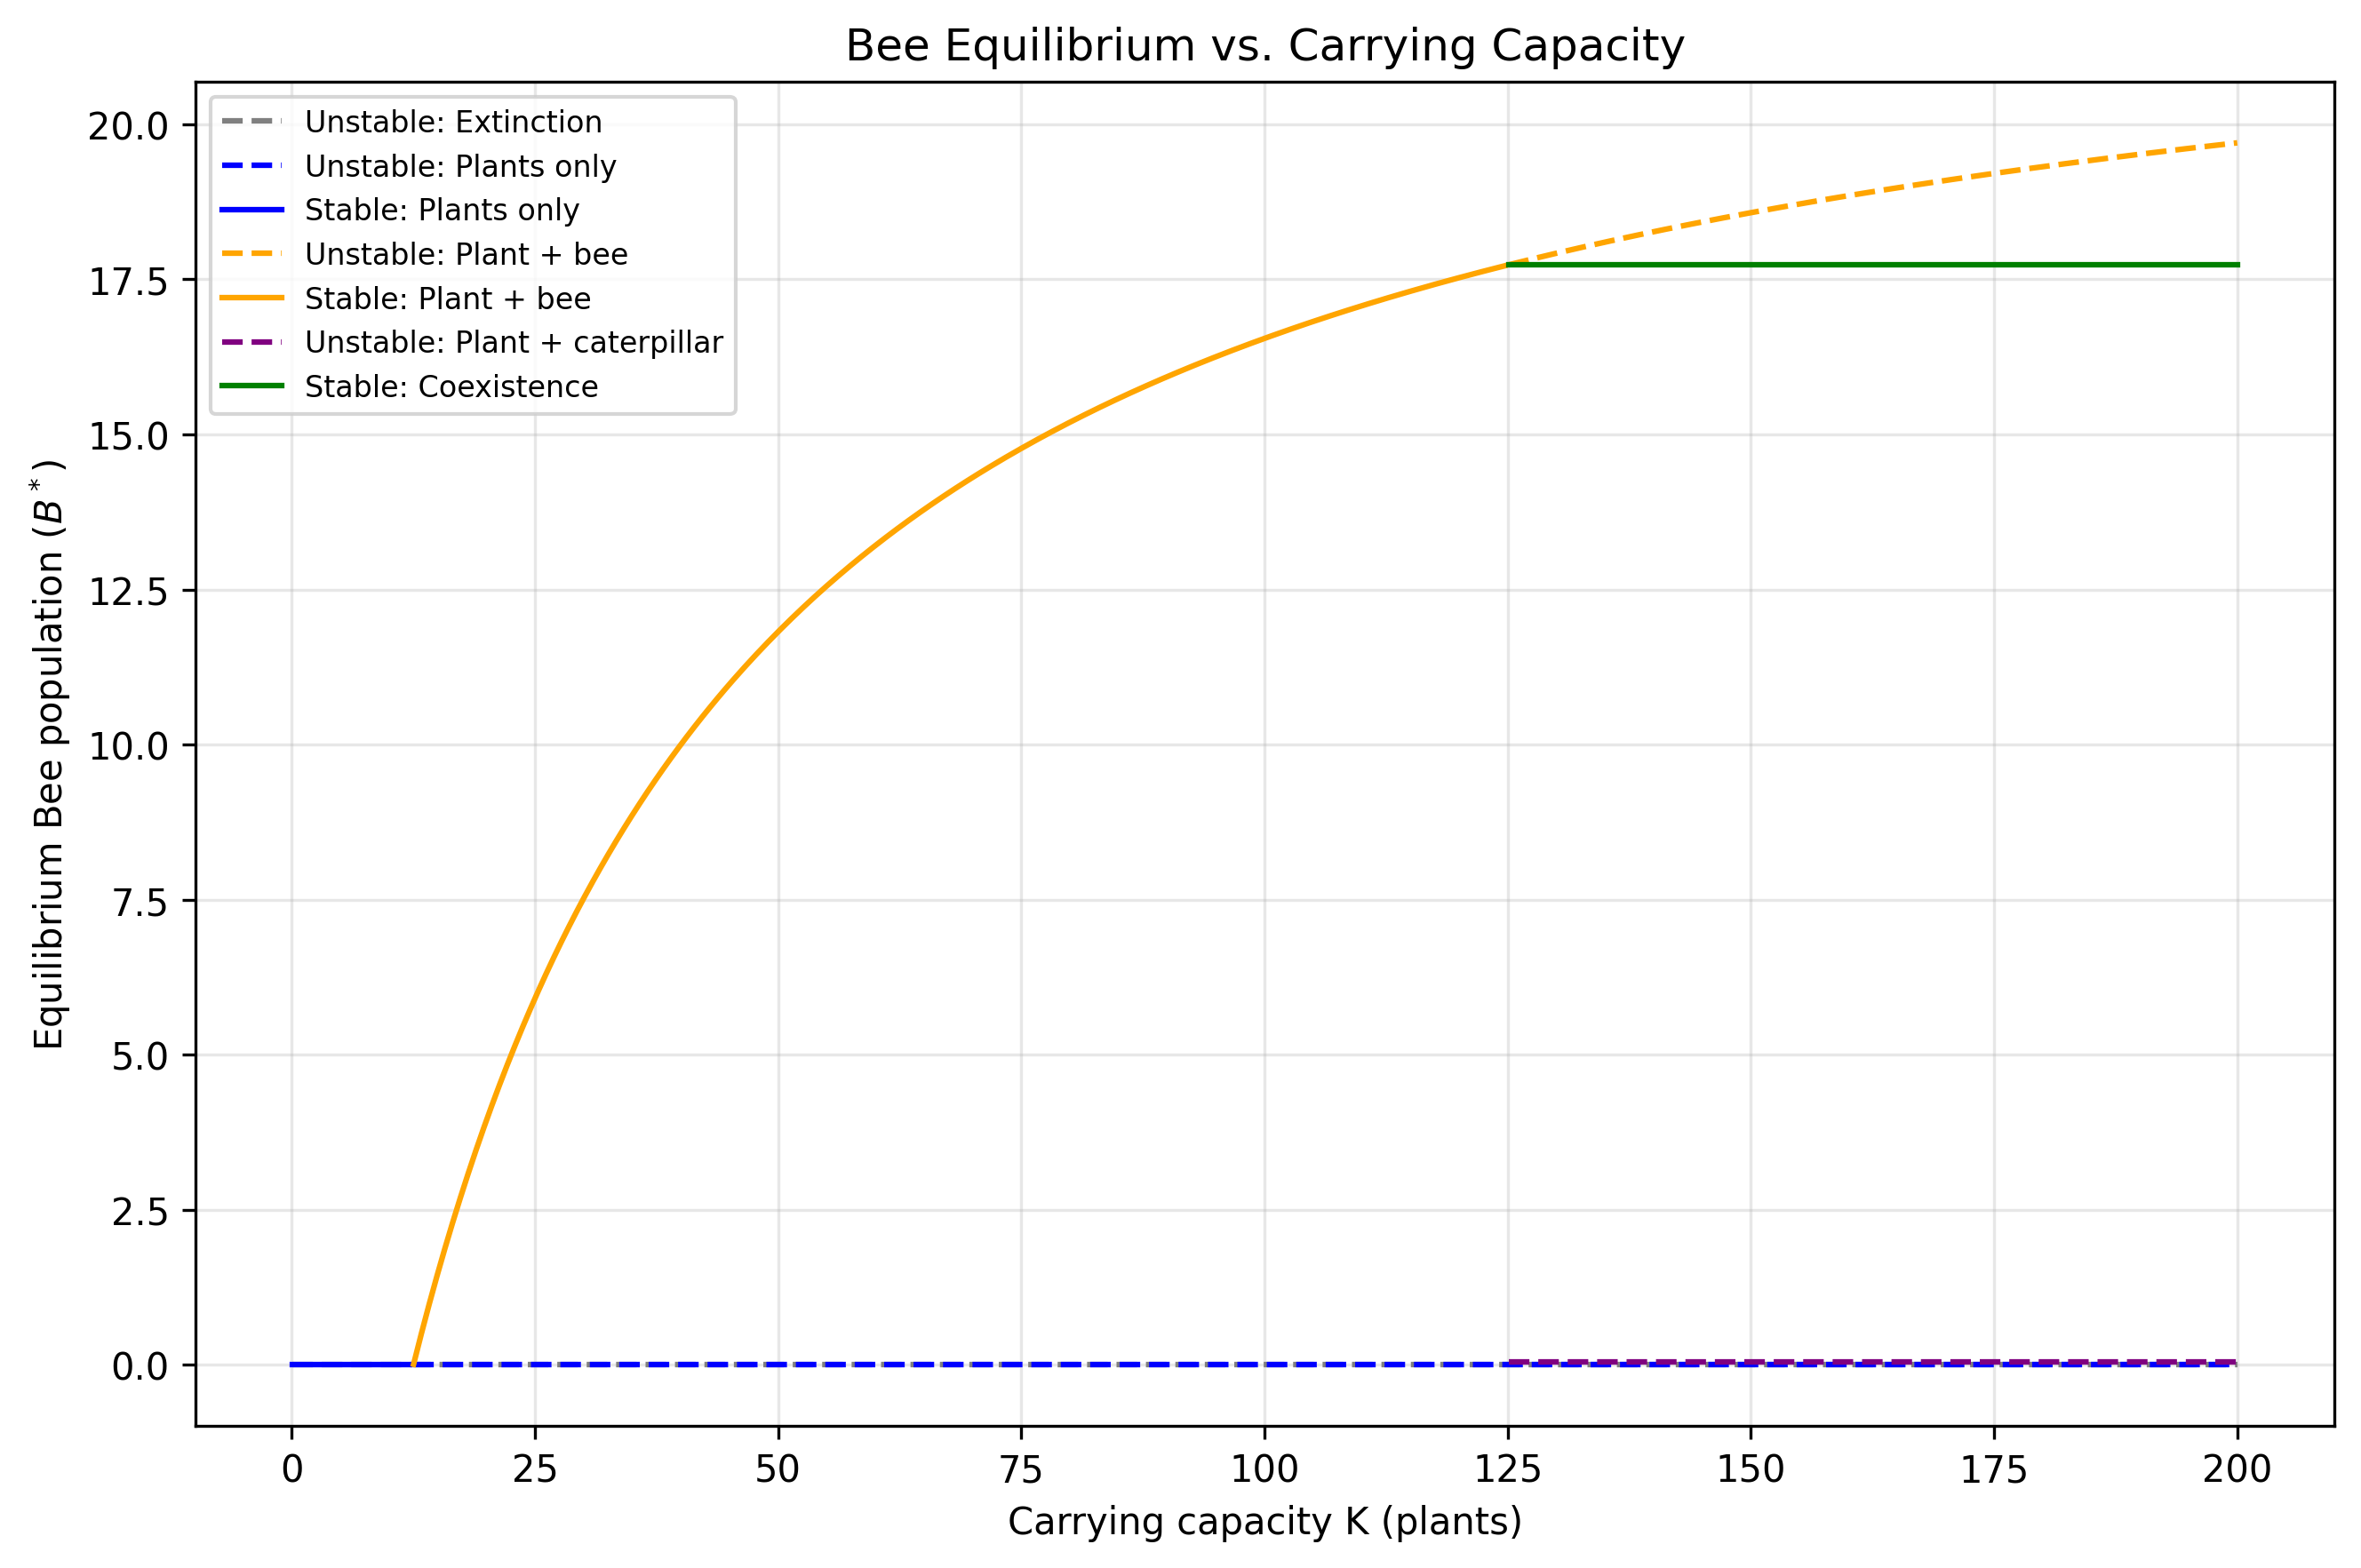
\includegraphics[width=0.48\textwidth]{model2_bees.png}

\caption{Bifurcation diagrams for Model 2 showing equilibrium plant (top left), caterpillar (top right), and bee (bottom) populations as plant carrying capacity varies. Solid lines indicate stable equilibria, and dashed lines indicate unstable equilibria. Small display offsets separate overlapping branches.}
\label{fig:model2-bifurcation}
\end{figure}

The bifurcation diagrams for Model 2 show how the equilibrium populations of plants, caterpillars, and bees change in both stability and existence as the plant carrying capacity ($K$) increases. Adding bees introduces two additional possible equilibria: coexistence between plants and bees (orange), and coexistence among all three populations (green).

For our chosen parameters, the plants-only equilibrium (blue) loses stability near $K=12.50$, allowing stable plant--bee coexistence. The plant--bee equilibrium then loses stability at $K=125$, allowing stable three-species coexistence. Over $125<K\leq200$, caterpillar abundance increases with carrying capacity, while plant abundance remains at 125 and bee abundance remains approximately constant. Interestingly, at $K=200$, both models predict 125 plants, but Model 2 supports approximately 43 caterpillars compared with 4 in Model 1. Bees support additional plant growth, allowing more caterpillars to survive; however, their increased consumption leaves the equilibrium number of standing plants unchanged.

\FloatBarrier

\clearpage
\subsection{Interventions}
\leavevmode\par

\begin{figure}[!htb]
\centering
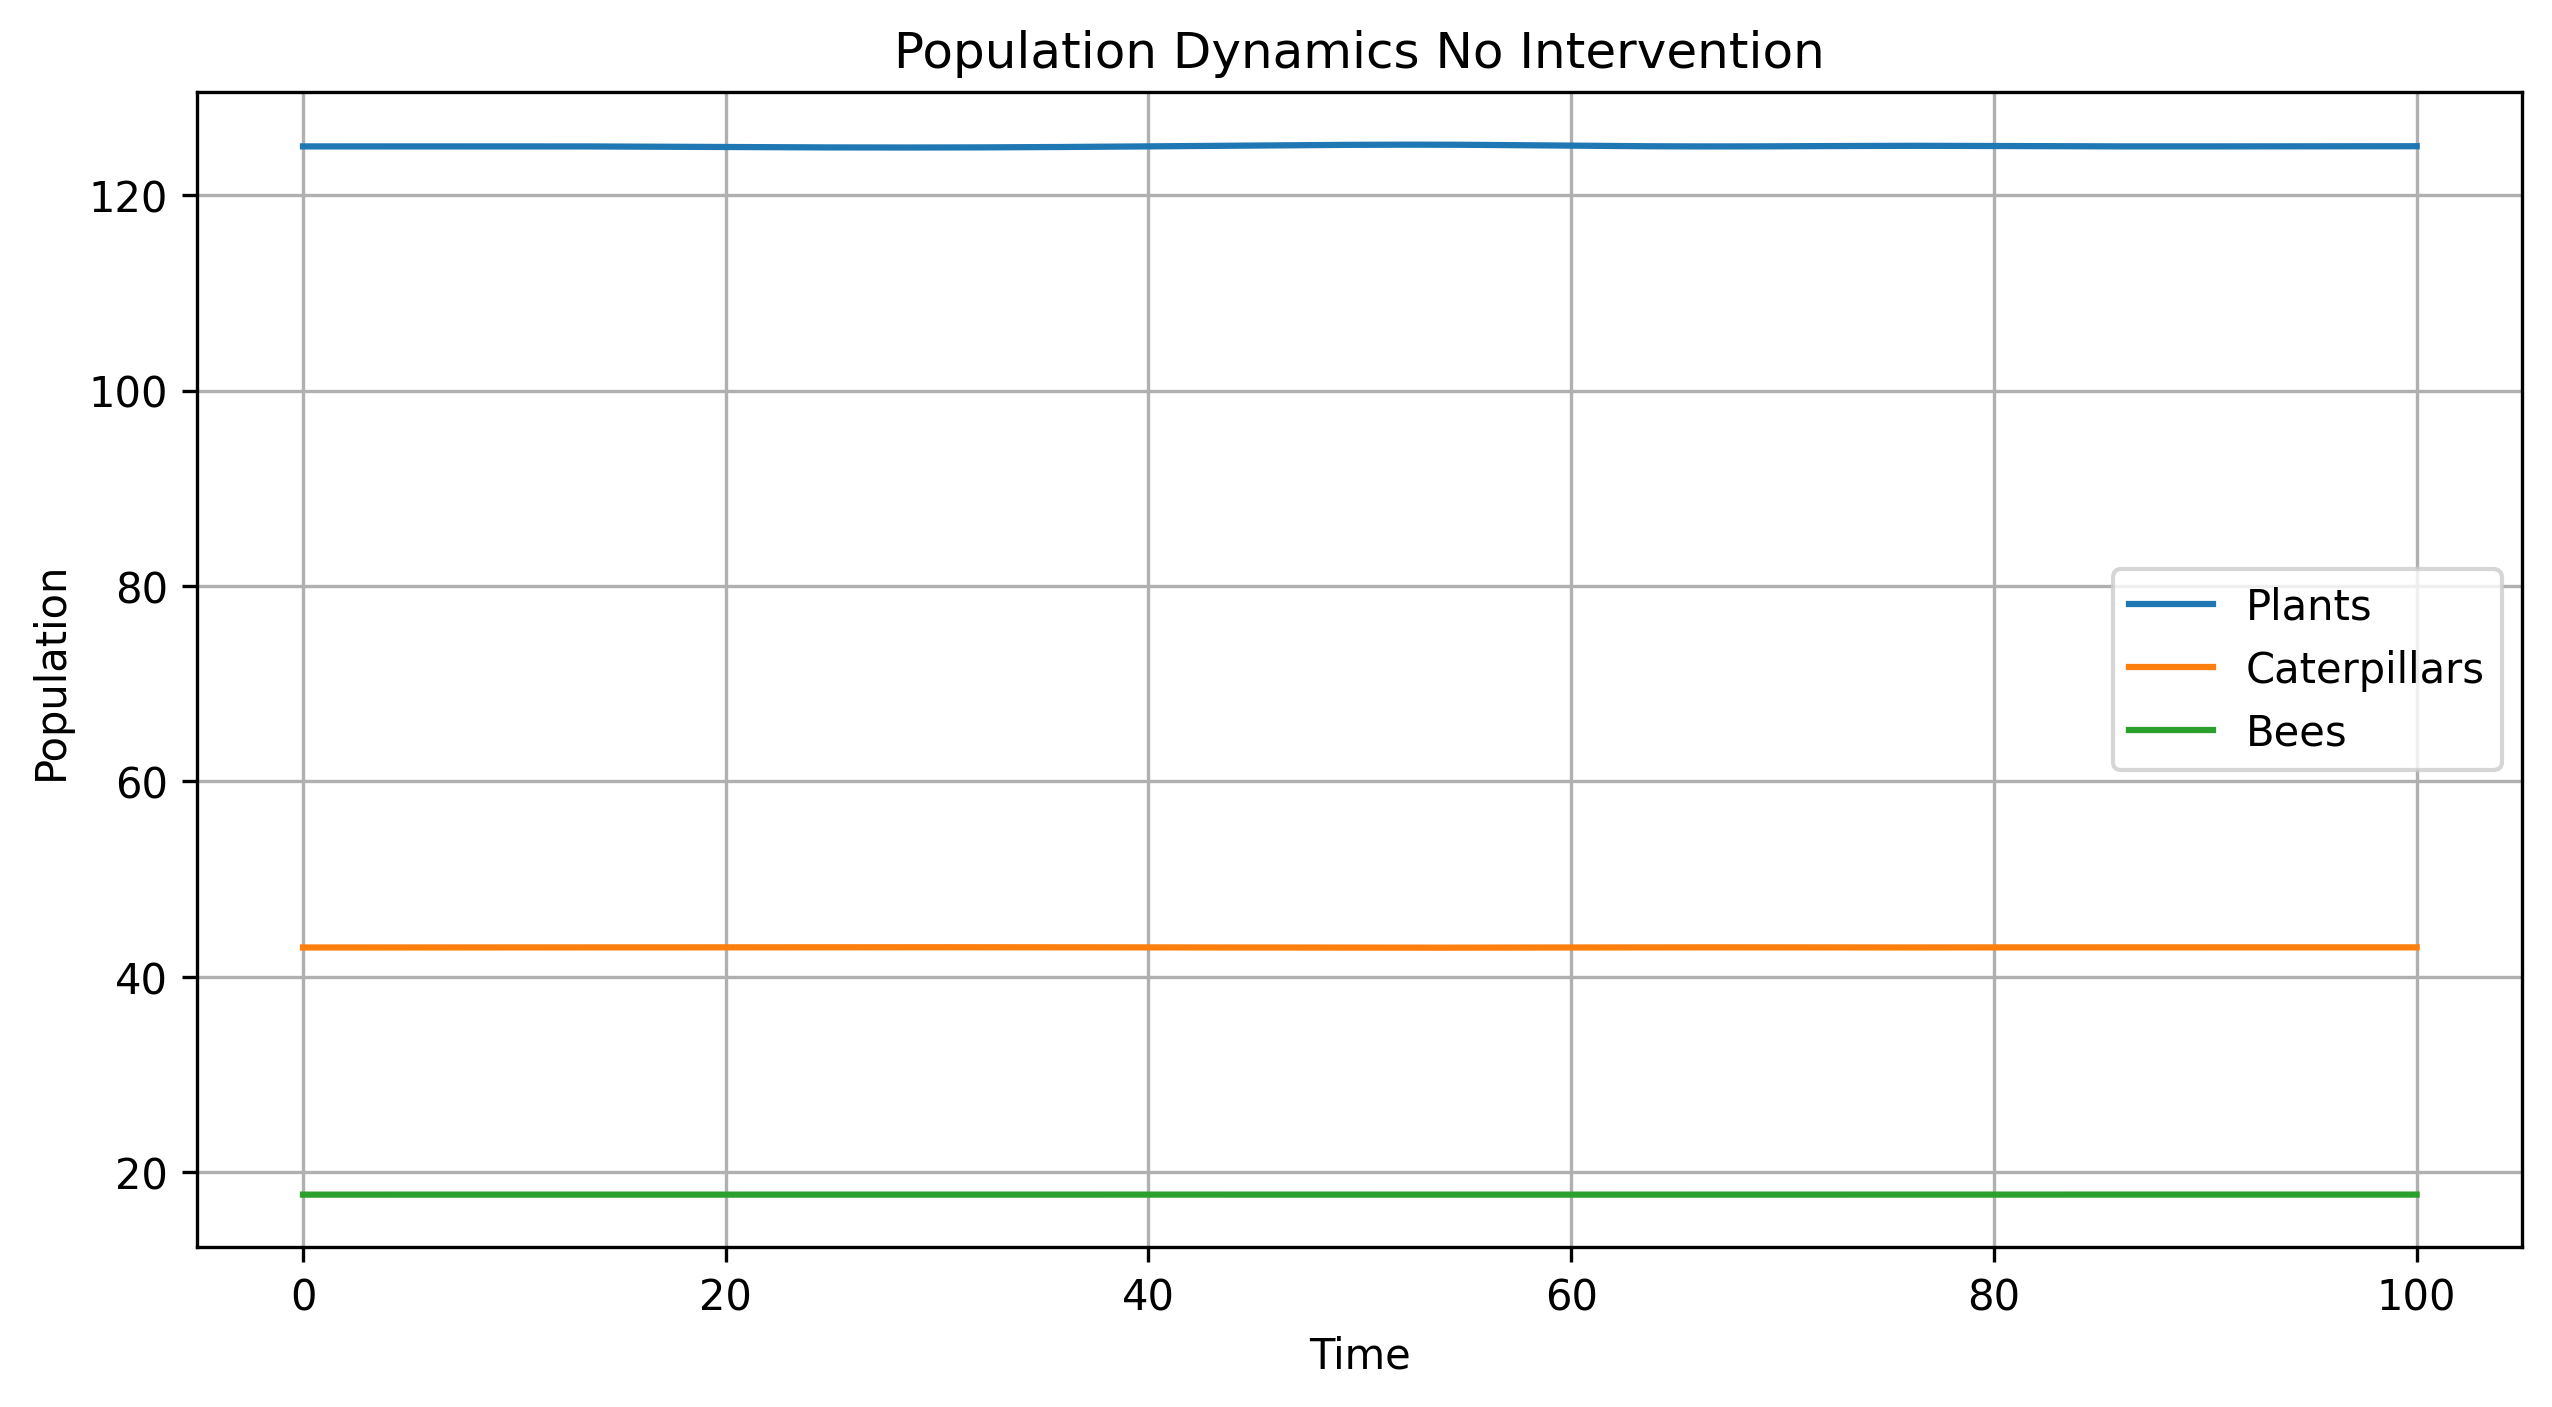
\includegraphics[width=0.72\textwidth]{Population Dynamics No Intervention.png}

\medskip
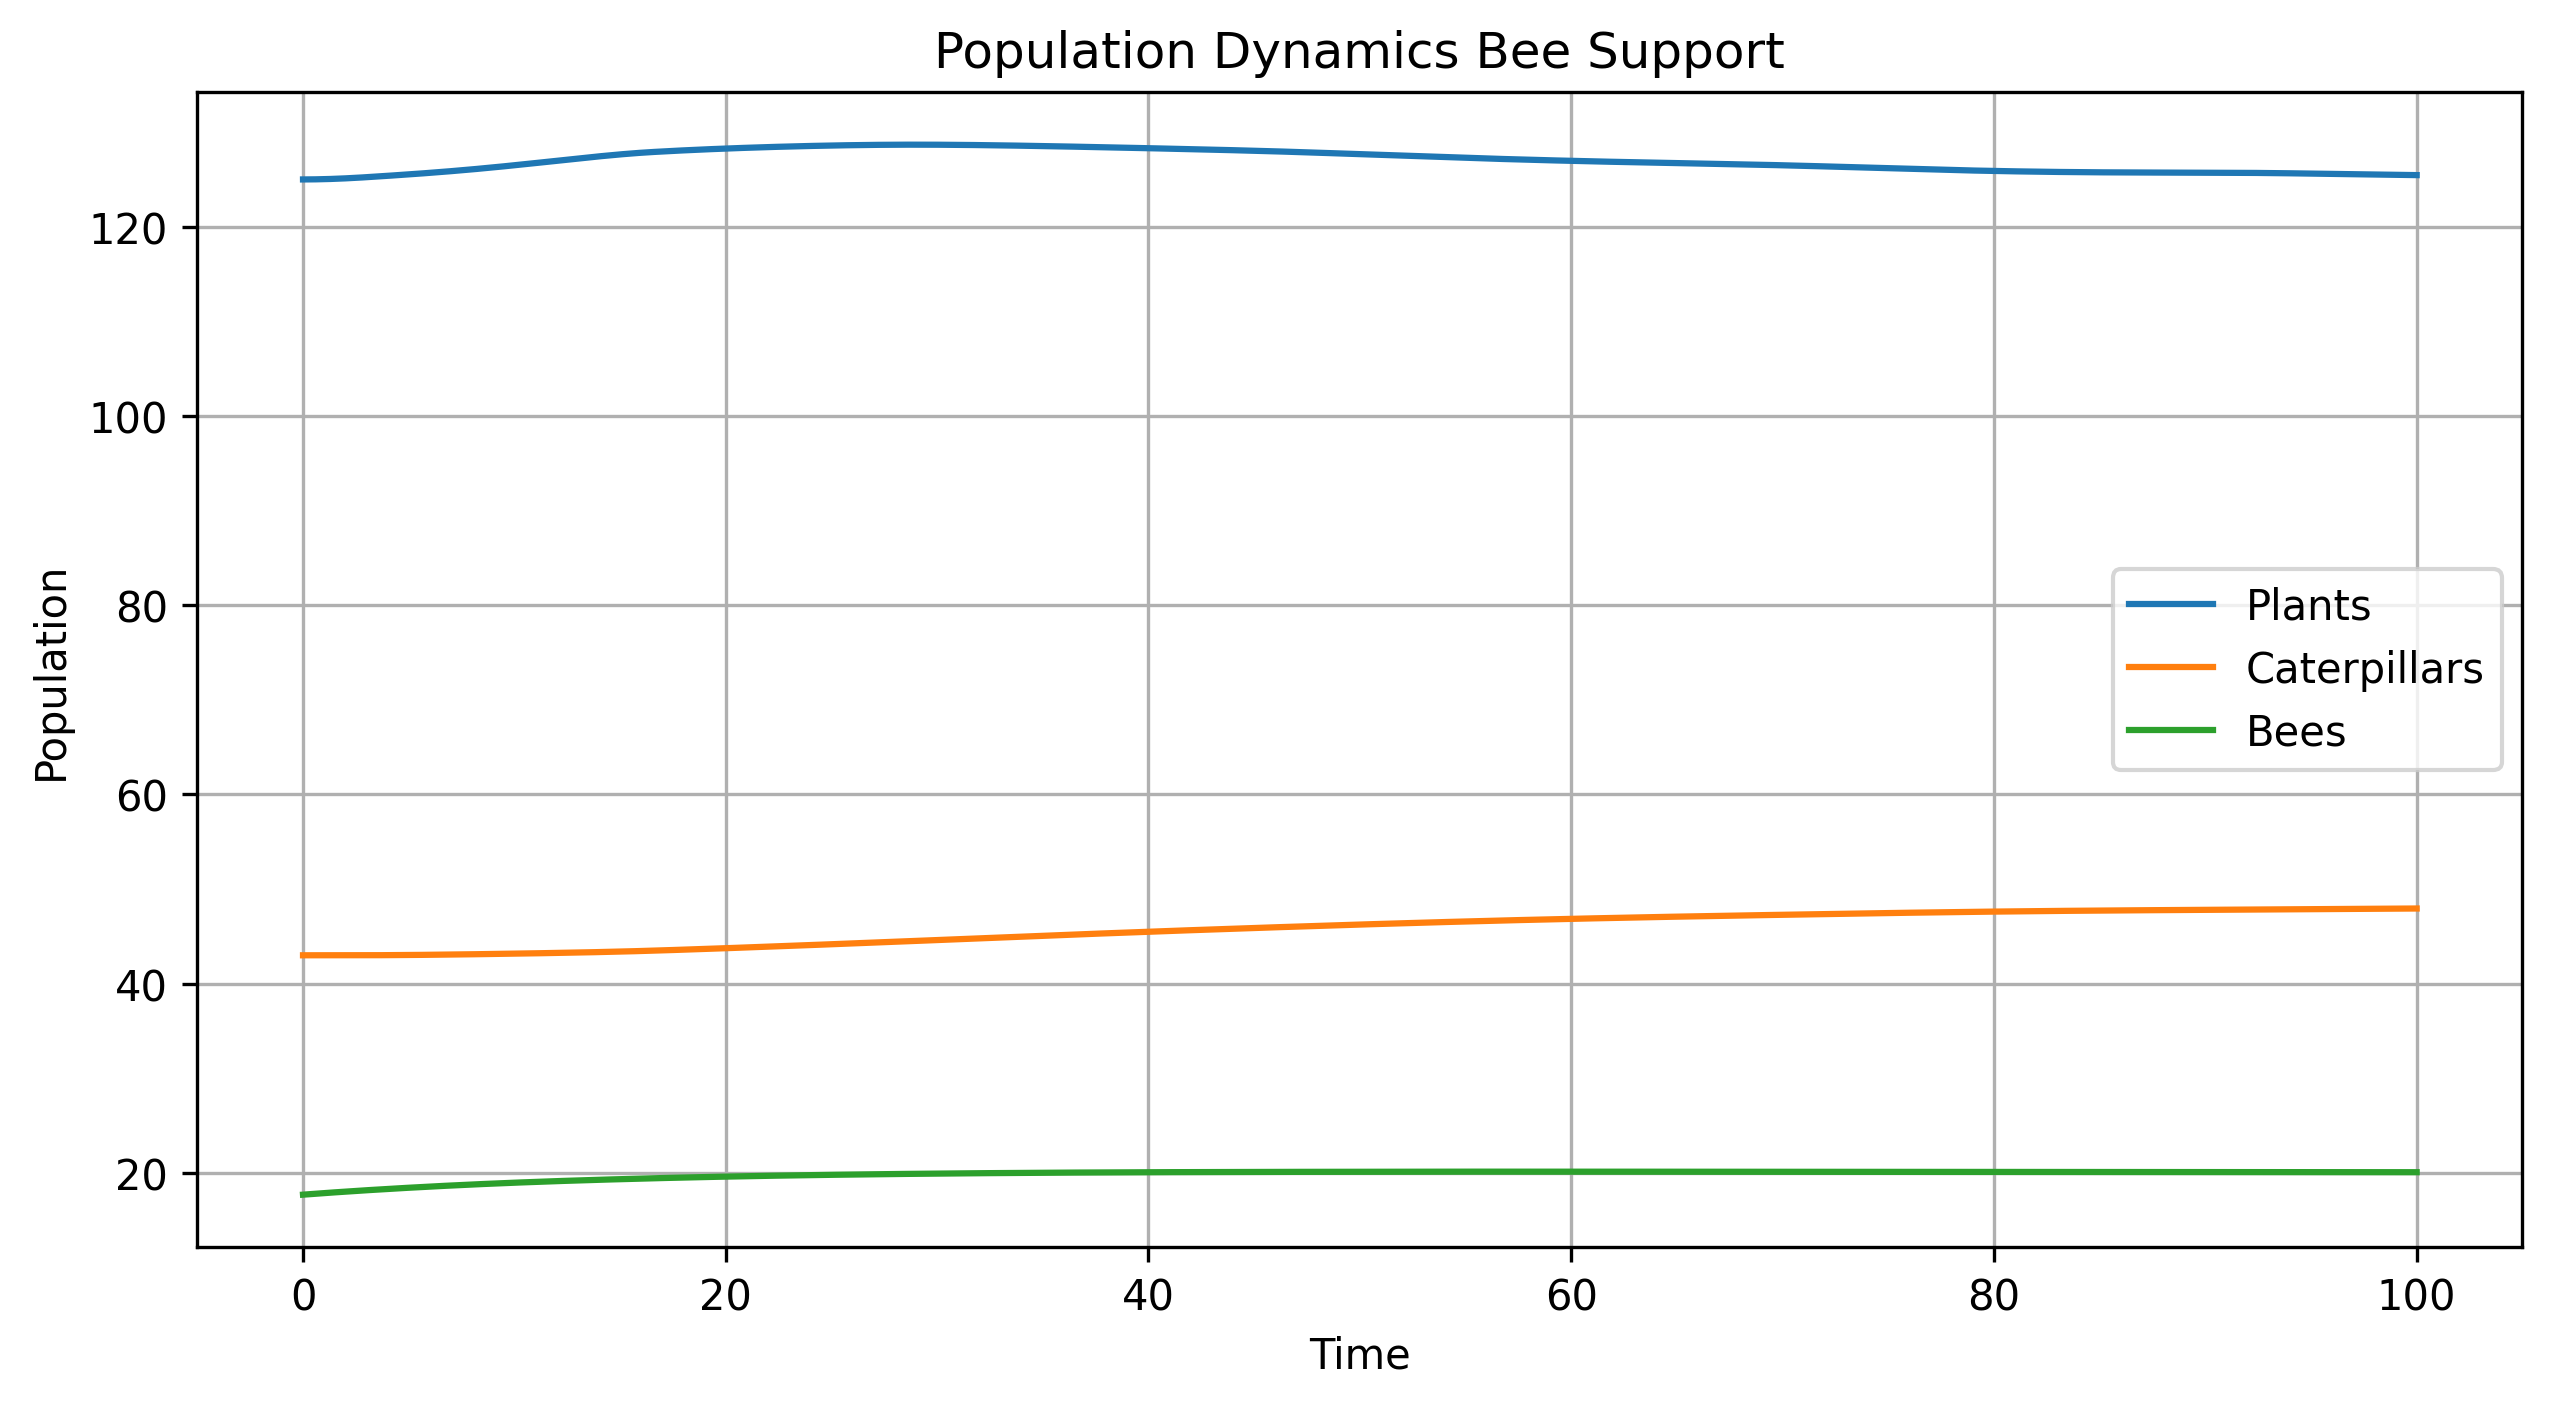
\includegraphics[width=0.72\textwidth]{Population Dynamics Bee Support.png}

\medskip
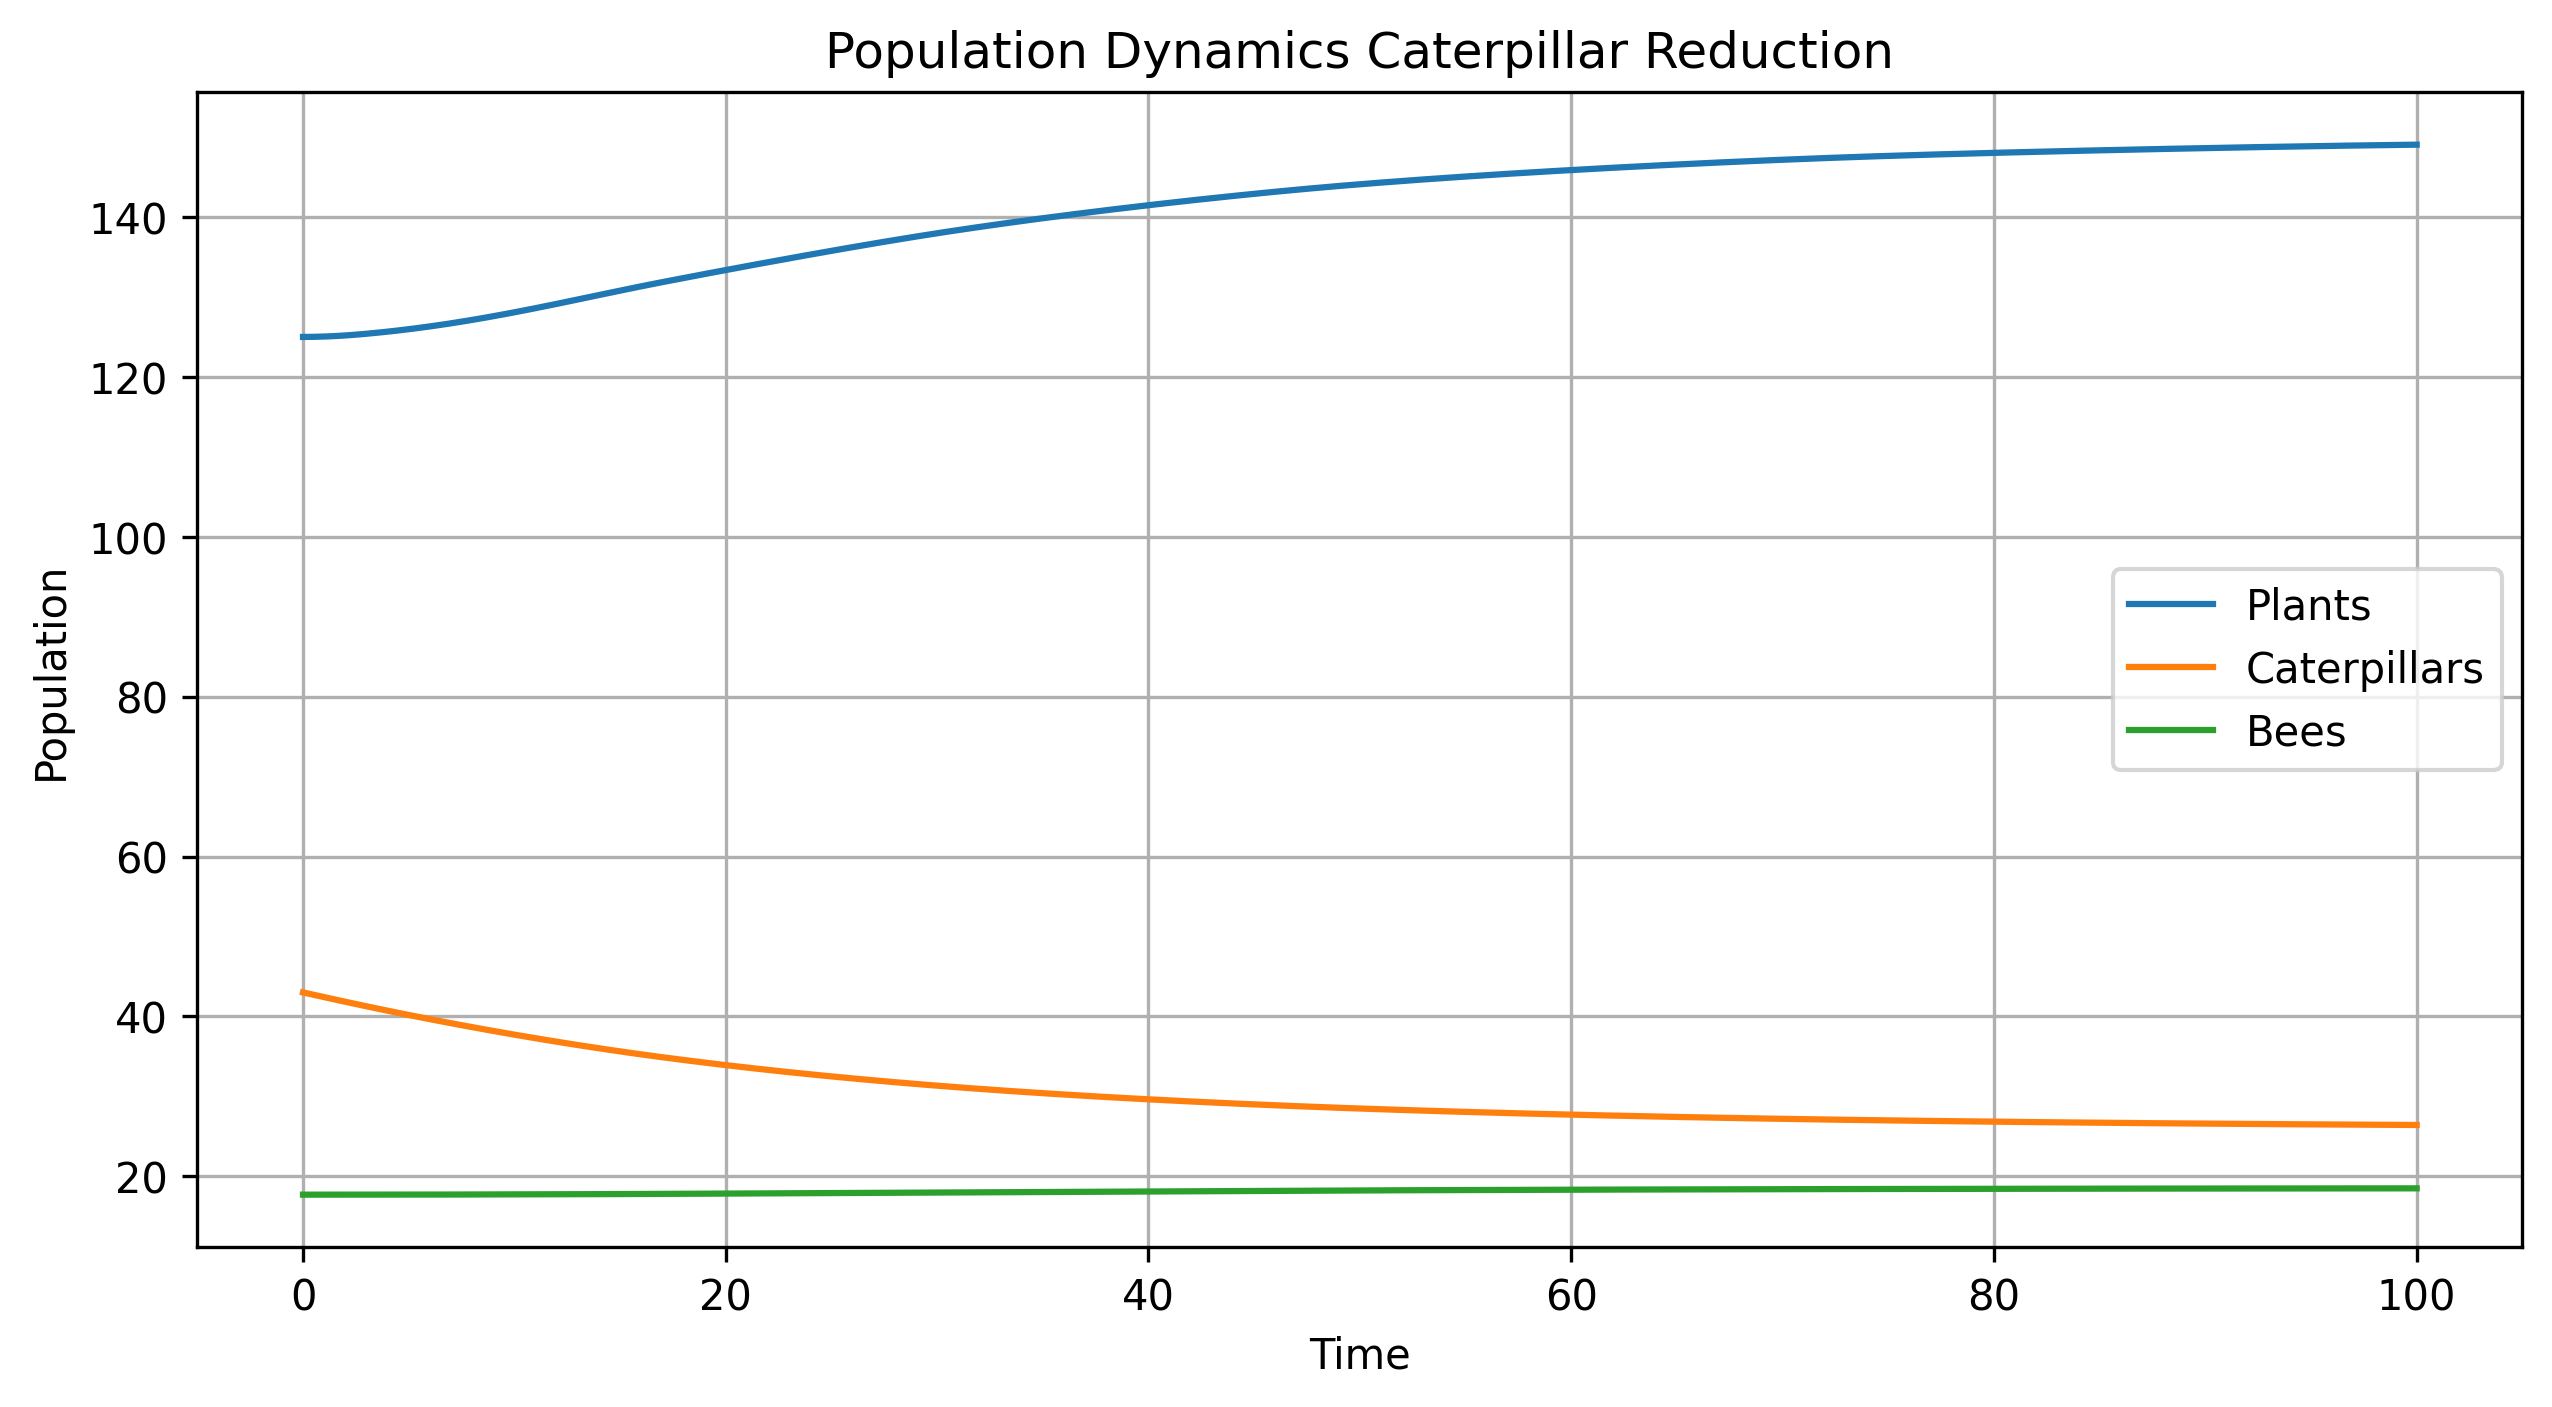
\includegraphics[width=0.72\textwidth]{Population Dynamics Caterpillar Reduction.png}

\caption{Model 2 population dynamics at $K=200$ with no intervention (top), bee support through a 20\% decrease in bee mortality (middle), and caterpillar reduction through a 20\% increase in caterpillar mortality (bottom). All simulations use the same initial populations.}
\label{fig:interventions}
\end{figure}

\FloatBarrier

Panel 1 of Figure~\ref{fig:interventions} shows the populations at the coexistence equilibrium. For our chosen parameters, this equilibrium at $K=200$ is stable. Thus without intervention, the populations remain at this equilibrium. We then ask whether we can increase the plant population through human intervention. The first intervention, represented by Panel 2, supports bees. In practice, this could involve reducing bees' exposure to harmful pesticides~\cite{epaPollinatorProtection}. In our model, we represent this by decreasing the bee mortality rate $d$ by 20\%. As seen in Panel 2, this results in a temporary increase in plant abundance, which then supports growth of the caterpillar population. As the caterpillar population increases, the plant population decreases and returns close to its initial level.

We then consider a second intervention, shown in Panel 3, that reduces caterpillars. In practice, this could involve encouraging natural predators of caterpillars as a form of biological control where herbivory is excessive~\cite{ucipmLeafFeedingCaterpillars}. We represent this by increasing the caterpillar mortality rate $\mu$ by 20\%. In Panel 3, as the number of caterpillars decreases, the plant population increases toward a higher level than its initial abundance. The caterpillar population decreases toward a lower level but remains positive. Caterpillars are therefore reduced rather than completely eliminated.

%%Fourth Section
\section{Analysis/Conclusions}

\subsection{Equilibria and Population Dynamics}

Our models demonstrated how interactions between plants, caterpillars, and bees influence the long-term behavior of an ecosystem. Model 1 successfully represented three possible outcomes: extinction of both populations, plants surviving without caterpillars, and coexistence between the two species. Adding bees in Model 2 introduced additional equilibria, including plant-bee coexistence and coexistence of all three species. This allowed us to explore a more complete set of possible population dynamics.

An interesting result was that adding bees allowed the ecosystem to support a much larger caterpillar population. At a carrying capacity of $K=200$, Model 1 predicted an equilibrium plant population of 125 and a caterpillar population of approximately 4. In Model 2, the plant population remained at 125, but the caterpillar population increased to over 40. This suggests that pollination can increase the resources available to caterpillars, resulting in higher caterpillar abundance without necessarily increasing the long-term equilibrium plant population. This is due to the increase in plant consumption by the larger caterpillar population. 

\subsection{Interventions}

Our simulations showed that supporting bees alone did not produce a lasting improvement in plant abundance. Although bees contribute positively to plant growth through pollination, their benefits were not sufficient to overcome the effects of caterpillar consumption. In contrast, reducing caterpillar populations improved plant abundance over the long term. This suggests that managing herbivore populations may be more effective than relying on pollinator support alone when the primary goal is maintaining plant populations. Caterpillars do not need to be eliminated entirely; reducing their population can be sufficient to improve plant survival.

\subsection{Limitations and Future Work}

Although our models captured several important ecological relationships, they simplified a much more complex ecosystem. We assumed constant growth, mortality, and interaction rates and did not account for seasonal changes, environmental conditions, or other species that could influence population dynamics. Although our parameter values were informed by published literature and biologically motivated estimates, we did not calibrate the model against observed population data from a specific ecosystem. With more time, we could incorporate real ecological data, investigate seasonal effects, and explore additional interventions.

Overall, this project helped us understand how systems of ordinary differential equations can be used to represent biological interactions and predict long-term population behavior. We also learned how equilibrium and stability analysis can help identify the conditions under which species can coexist. While our models cannot capture every aspect of a real ecosystem, they provide useful insight into how plants, caterpillars, and bees depend on one another and how different strategies of managing the ecosystem can influence their populations.

\section{AI Disclosure}

AI was used in the following ways on this project: AI was used to search for potential datasets and research sources, work through errors in code, and check equilibrium calculations to see if they were realistic.

AI was not used to write the text of the report, develop the models, nor analyze and evaluate our models, except as a peer reviewer after we had already submitted our draft for peer review.

%%%%%%%%%%%%%%%%%%%%%%%%%%%%%%%%%%%%%
%% Bibliography below
%%%%%%%%%%%%%%%%%%%%%%%%%%%%%%%%%%%%%
\FloatBarrier % Keep the figures from being put after the bibliography
\newpage
%% If using bibtex, leave this uncommented
\bibliography{refs} %if using bibtex, call your bibtex file refs.bib
\bibliographystyle{unsrt}

%% If not using bibtex, comment out the previous two lines and uncomment those below
%\begin{thebibliography}{99}
%\bibitem{Vandermeersch} First reference goes here
%\end{thebibliography}

\end{document}
